\begin{fullwidth}
\chapter{\label{ch:super_methods}
The syllables superposition experiment}
\end{fullwidth}

\begin{chabstract}

In this chapter we present the two tasks of the experimental design, the Bold-fMRI data acquisition, preprocessing and processing, and the analysis methods employed to assess the likelihood of superposed representations in the Regions of Interest considered.

\end{chabstract}

\section{Experimental design}

\paragraph{Participants:}
Five native French speakers participated in the experiment (two females with ages 22 and 32 and three males with ages 23, 26 and 36).
All subjects had high school background from French universities (Bac) and were right handed with a Laterality Quotient (LQ) of at least 40 (mean 70, SD 20.98), as measured by the Edinburgh Handedness Inventory\citep{oldfield1971assessment}.
The experiment was sponsored by the language neuroimaging unit of Unicog lab U-992 in NeuroSpin, and received ethical approval by the regional ethical committee (Comite de Protection des Personnes, hopital de Bicetre).
All subjects gave written informed consent and received 80 euros for their participation.

\paragraph{Introduction to the experimental design:}

Two tasks were implemented for the experiment;
a language localizer task, well explored and validated in the literature\citep{mahowald2016reliable}, to identify in each subject language processing regions, and a pseudoword matching task to obtain brain representations of syllable permutations.
All experimental tasks were implemented with python scripts exploiting the capabilities of the Expyriment python library\citep{krause2014expyriment}.

For both tasks, visual and auditory sensory modalities were used for stimulation, since in language regions we aim to find abstract representations insensitive to sensoty modality.
Visual Stimuli consisted of text, projected one word at a time in rapid serial visual presentation (RSVP), on a translucent screen with a digital light processing projector (PTD7700E, panasonic, frame rate: 60 Hz, resolution of 1024 x 768), with a viewing distance of 89 cm.
Auditory Stimuli were delivered through MRI-compatible headphones (MR confon), and the volume was adjusted for each participant to a comfortable hearing level.


\subsection{Language Localizer}

\paragraph{Stimuli:}
The stimuli consisted on blocks of three phrases and blocks of three non word sequences that varied in implementation with the sensory modality.
These blocks were presented in an alternated fashion with the purpose of extracting brain areas processing language from the contrast of these block categories\citep{mahowald2016reliable}.
Visual stimuli was text presented in the screen with a fixed point Inconsolata font\footnote{https://fonts.google.com/specimen/Inconsolata}.
The text comprised 0.72 degrees of vertical visual angle and a maximum of 5.8 degrees of horizontal visual angle, with the longest word having 14 letters.
The visual non words stimuli was formed by replacing words in the phrases with consonant strings, for example "the cat" would be replaced by "ztr pfg".
Auditory stimuli consisted on the same phrases digitally recorded at 22.05 kHz in a quiet room by a male speaker.
Phrase recordings had a mean duration of 2.33 seconds (SD, 0.41 s), giving a total average duration of 7 seconds for a block made of three sequences.
To generate the control auditory non word sequences, the phrase recordings were scrambled with the multiband approach suggested by Ellis and Lee\citep{ellis2010time}, but with python code using the Brain Hears software\citep{fontaine2011brian}.

\paragraph{Task and trial structure:}
The subjects were instructed to read or listen to the word sequences and pay attention to the non word sequences.
Each trial consisted on presenting one of the blocks designed, which were phrases or non words.
Each block made of word and non word units contains three sequences, the first sequence made of 9 units, the second of 10 units and the last of 9 units.
A fixation cross would be presented before the presentation of each sequence, for 500 ms, followed by a blank screen for 500 ms.
In the visual case, each text unit would be presented regularly for 200 ms, which is not the case in the audtiory modality that has variable sequence duration.
Between the presentation of the three different sequences a blank screen would be presented for 600 ms.
At the end of the presentation of the three sequences a blank screen would be presented for 7 seconds waiting for the next trial (the next block).
There were 4 runs of acquisition and in each of them 90 trials were
presented.
In Figure \ref{fig:langlog_trial} we show an example of a sequence in the visual modality.

\begin{figure*}[hptb]
\centering
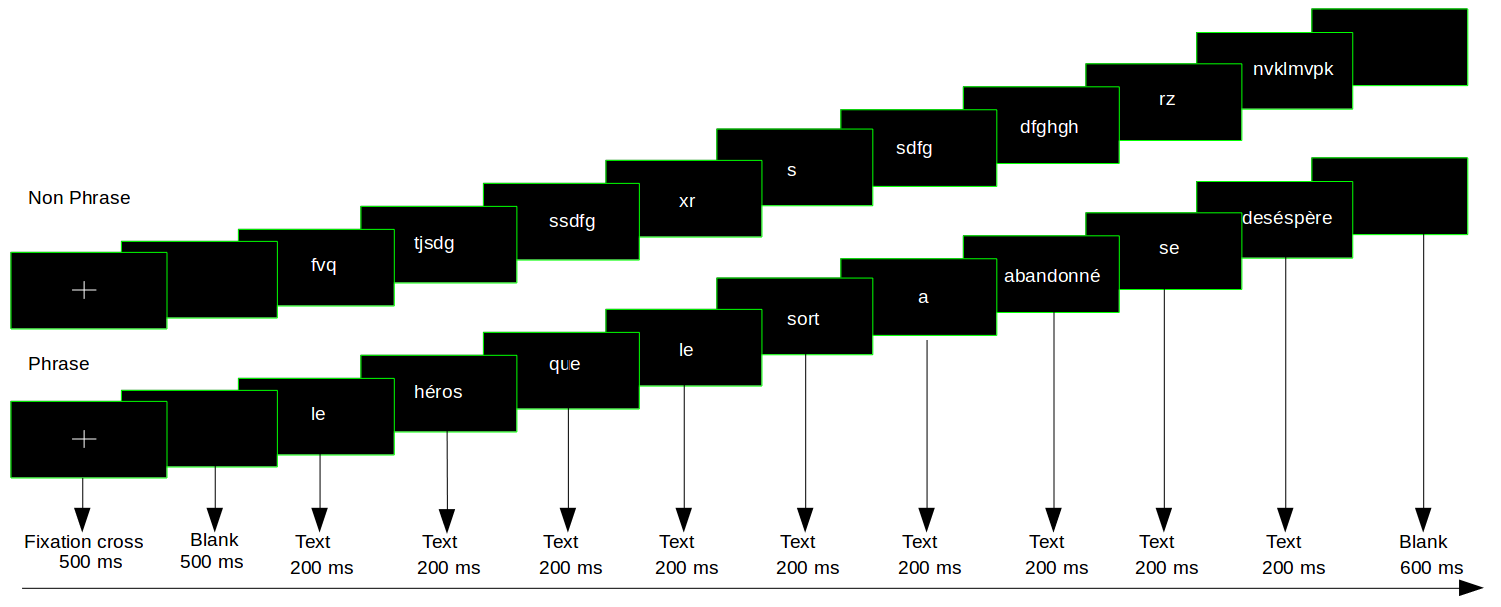
\includegraphics[width=1.0 \linewidth]{figures/part_II/langloc_trial.png}
\caption{\textbf{Visual trial of the language localizer:}
Each black square represents the screen at a different time point.
Only one example word and non word (consonant string) sequence is shown, which comprises only one third of a block stimuli.
}
\label{fig:langloc_trial}
\end{figure*}


\subsection{Pseudoword matching task}

% Stimuli
\paragraph{Stimuli:}
The syllables "fi", "gu" and "na" were selected to form all the possible pseudoword permutations "fifi", "figu", "fina", "gufi", "gugu", "guna", "nafi", "nagu" and "nana".
These syllables were selected under two constraints.
The first was that all syllabic combinations would not lead to word formation, such that we could assume similar sensory and language processing of symmetric representations like "figu" and "gufi", expecting only syllable position effects.
The second was that we wanted to improve auditory discriminability, so we selected one velar consonant "gu", one labio-dental "fi" and one alveolar "na" with their respective high-back tongue "u", high-front tongue "i" and low-back tongue "a" vowels.
We based this heuristic on the phonetic organization of spatial patterns demonstrated in the cortex by Bouchard et al\citep{bouchard2013functional}.

The pseudowords were presented in a visual and auditory modality.
In the visual case they were presented as text in the screen with a fixed point Inconsolata font.
We decided to make the text as big as possible to increment expected retinotopic effects but also tried to avoid the stimuli perception to be unnatural and too tiring for the subjects, so finally the pseudowords were presented as lowercase text centered on the screen, spanning maximum 2.39 degrees of vertical visual angle and maximum 5.05 degrees of horizontal visual angle.
In the auditory case each syllable was digitally recorded at 22.05 kHz in a quiet room by a male speaker and then the recordings were combined to produce with a 660 ms duration all the possible pseudowords having identically pronounced syllables in each position.
The matching task was not constant across trials, so we decided to make a clear distinction between the target and probe stimuli.
Then we presented smaller uppercase text spanning 0.6 degrees of vertical visual angle and 1.68 degrees of horizontal visual angle for the visual modality and modified recordings of the syllables with higher pitch for the auditory modality.


\paragraph{Task and trial structure:}
The task consisted on keeping the pseudowords in memory for a possible comparison with a second pseudoword.
The exact instruction given to the subjects was to fixate a green dot that would signal appearance of the pseudoword that had to be kept in memory until the arrival of a red dot that signaled the end of the trial.
The subjects were instructed to keep paying attention to the screen or sound for a second pseudoword that would appear only in some randomly selected trials, in which case, confirmation of a positive match would be done with a right hand button press and of a negative match with a left hand button press.
We included the matching task to validate subjects were paying attention to the stimuli, but we did not include a matching task on each trial to try to maximize the amount of stimuli presented in a session.

The green dot appeared for 0.5 seconds followed by a flashing presentation of the pseudoword, in the visual case, to be kept in memory for 3.2 seconds with a 0.25 seconds jitter.
We decided to present the visual pseudowords for only 0.2 seconds to minimize the influence of saccades in the estimation of brain activations.
In the matching task trials, the second pseudoword was presented for 0.5 seconds followed by a response and rest period of 6.5 seconds.
At the end of the trial the red dot was presented for 0.5 seconds followed by a 2.5 seconds resting period.
Each imaging run consisted of 45 trials (5 per pseudoword), where the order of presentation of the pseudoword conditions was shuffled.
In total there were 8 runs in a session, with two auditory sessions and two visual sessions, for a total of 80 trials per condition per modality.
Only nine trials were randomly selected to contain a second pseudoword to perform a matching task.
We show the structure of a trial from the visual modality in Figure \ref{fig:syllable_trial}.
In the auditory case the trial structure is identical except for the 660 ms duration of the pseudowords recordings, in which case the memory time was reduced to 2.8 seconds to have the same trial total duration as in the visual case.


\begin{figure}[hptb]
\centering
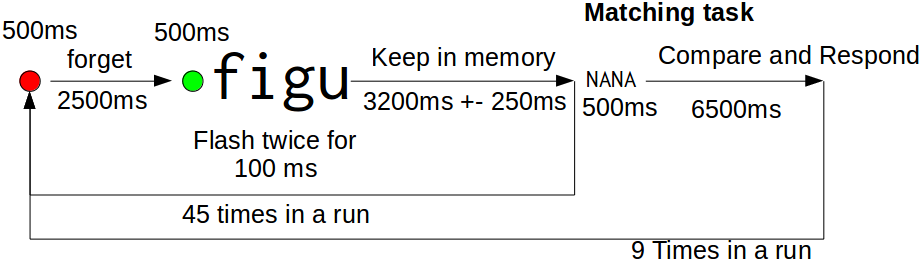
\includegraphics[width=1.0 \linewidth]{figures/part_II/syllable_trial.png}
\caption{\textbf{Visual trial example of the pseudoword matching task:}
A green dot is presented for 500 ms, followed by a pseudoword flashed twice for a total presentation duration of 200 ms.
It has to be kept in memory for a period of 3200 ms with a 250 ms jitter.
Nine times in a run a second uppercased pseudoword is presented for comparison during 500 ms with a response period of 6500 ms.
}
\label{fig:syllable_trial}
\end{figure}


\section{Data acquisition and processing}

\paragraph{Imaging:}
The acquisition was performed with a 3 Tesla Siemens Prisma Fit system equipped with a thirty two channels coil.
Anatomical images were taken using a 3D Gradient-echo sequence and voxel size of 1x1x1 mm.
Functional images were acquired as T2*-weighted echo-planar image volumes (Multi-Band EPI C2P from Minnesota University).
The MultiBand EPI consisted on the parallel acquisition of 4 slices at a time, reconstructed by a parallel imaging reconstruction algorithm\citep{chaari2011wavelet}.
Eighty transverse slices covering the whole brain were obtained with a TR of 1.5s and a voxel size of 1.5 x 1.5 x 1.5 mm (TE = 26.8 ms, flip angle = 70, no gap).
Moreover accurate timing of stimuli presentation relative to FMRI acquisition was achieved with an electronic trigger at the beginning of each run.

\paragraph{Acquisition sessions:}
Each subject had four sessions of scanning with a similar structure.
The first two sessions included the visual version of the pseudoword matching task and the last two sessions the auditory version.
Each scanning session lasted 78 min and 6 sec with an anatomical scan and 10 functional runs structured as follows:

\begin{enumerate}[leftmargin=1.5cm, itemsep=-0.12cm, topsep=0.25cm]
\item Anatomical T1 (1 volume, 7m 46s)
\item Pseudoword matching task "Visual/Auditory" (253 volumes, 6m 54s)
\item Pseudoword matching task "Visual/Auditory" (253 volumes, 6m 54s)
\item Pseudoword matching task "Visual/Auditory" (253 volumes, 6m 54s)
\item Pseudoword matching task "Visual/Auditory" (253 volumes, 6m 54s)
\item Language localizer task "Visual" (435 volumes, 11m 27s)
\item Pseudoword matching task "Visual/Auditory" (253 volumes, 6m 54s)
\item Pseudoword matching task "Visual/Auditory" (253 volumes, 6m 54s)
\item Pseudoword matching task "Visual/Auditory" (253 volumes, 6m 54s)
\item Pseudoword matching task "Visual/Auditory" (253 volumes, 6m 54s)
\item Language localizer task "Auditory" (435 volumes, 11m 27s)
\end{enumerate}

% Preprocessing
\paragraph{Data preprocessing:}
The OASIS-30 Atropos template atlas from Mindboggle\footnote{http://www.mindboggle.info/data.html} was used as reference for normalization and segmentation of the subjects anatomy. The methodology behind this atlas is based on state of the art algorithms from the Advanced Normalization Tools (ANTS) and a cohort of 101 manually segmented subjects, giving very precise probabilistic maps and anatomical ROIs\citep{klein2005mindboggle}. A transformation between this template and one provided by ICBM in MNI space was also performed for MNI coordinate reports and visualization. The ICBM 2009a Nonlinear Asymmetric template was considered\citep{collins1999animal+}.

After normalization and segmentation of each subject anatomy. The functional runs of all tasks were slice timed with SPM with reference to the 1st slice (default SPM behavior) and realigned with respect to the 3rd volume of the first acquired run of the first session.
Realignment was performed with FSL MCFLIRT algorithm and coregistration was also performed with FSL but with the FLIRT algorithm employing a boundary based registration that takes into account previously performed white matter segmentation of the anatomy\citep{greve2009accurate}.
All preprocessing steps were implemented with the Nipype software\citep{gorgolewski2011nipype}.

\paragraph{Data processing:}
Two General Linear Model (GLM) estimations were performed, one on the non-smoothed, non-normalized and realigned functional images and the second on the smoothed version of the same images, with 6 mm gaussian kernel.
The GLM was implemented with the Nistats\footnote{https://github.com/nistats/nistats} software, which is part of the Nipy and Nilearn\citep{abraham2014machine} ecosystem.
A glover HRF was employed for the estimation with an additional cosine drift model to high-pass filter above 1/128Hz.

The language localizer was modelled with two regressors for the block conditions, alongside motion regressors extracted from the realignment preprocessing step.
Statistical estimation of a contrast between the two block conditions was performed on the smoothed images to extract the language network.

In the case of the pseudoword matching task, each pseudoword condition was modelled with one regressor, alongside left and right motor events derived from the behavioral responses and motion regressors extracted from the realignment preprocessing step.
The condition beta maps corresponding to the smoothed images were employed for statistical estimation of motor contrasts and syllable position effects, for which a fixed effect model was considered across runs and sessions in each subject.
To obtain statistical effects of syllable position, we modelled the conditions as two factors (left and right position), with three levels (syllables fi, gu and na).
We estimated contrast vectors for the effect of left position, effect of right position and interaction of left and right positions, by employing the contrasts vector specification procedure of Henson and Penny\citep{henson2003anovas}.

It has been shown that taking into account trial-to-trial variability is desirable for multivoxel pattern analysis (MVPA)\citep{abdulrahman2016effect, mumford2012deconvolving}.
As we wanted to look into the representational patterns of the different pseudowords, we decided to also estimate one beta map per trial, following the same methods employed for beta-series analysis\citep{cisler2014comparison}.
This is also desirable to capture attention modulated variability in the voxel patterns of the pseudowords, since the task do not allow us to verify the processing integrity of each trial but only to motivate subjects engagement.


\section{Data analysis}

All data analysis was performed employing diverse Python scientific open source libraries\ref{oliphant2007python}: Numpy\ref{walt2011numpy}, Pandas\ref{mckinney2010data}, Matplotlib\ref{hunter2007matplotlib}, Ipython\ref{perez2007ipython}, Scikit-Learn\ref{pedregosa2011scikit} and the neuroimaging library Nilearn\ref{abraham2014machine}.

\subsection{Regions of Interest (ROIs)}

\paragraph{Sensory-Motor regions:}
In Figure \ref{fig:sensory_example_img} we display the contours of primary sensory-motor regions, taken from the cytoarchitectonic SPM toolbox\citep{eickhoff2005new}, projected on the anatomy of Subject 1 alongside the gray matter mask.
Notice that the primary regions are broad, since we considered any voxel with non zero probability as part of the region, and cover both hemispheres.


\begin{figure}[hptb]
\centering
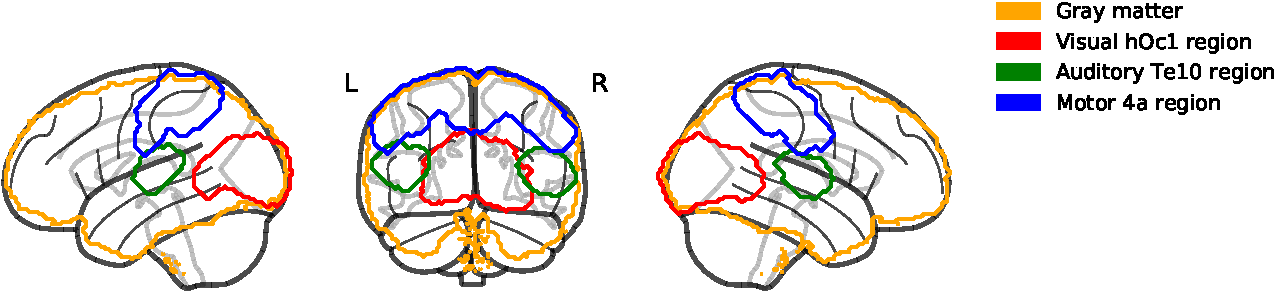
\includegraphics[width=1.0 \linewidth]{figures/part_II/sensory_example_img_with_legend.pdf}
\caption{\textbf{Sensory-motor regions projected on \emph{Subject 1} anatomy:}
Contours are shown for the projected primary Visual, Auditory and Motor regions, alongside the subject extracted gray matter.
}
\label{fig:sensory_example_img}
\end{figure}


\paragraph{Language regions:}
In Figure \ref{fig:fedorenko_example_img} we display the contours of the language localizer parcels derived by Mahowald and Fedorenko\citep{mahowald2016reliable}, that will be employed to evaluate the quality of the language localizer contrasts.
Then in Figure \ref{fig:langrois_example_img} we display the contours of left hemispheric language regions of interest taken from the Pallier et al. experiment in which phrase constituency effects were detected\citep{pallier2011cortical}.
We also show the joint Broca 44 and 45 regions taken from the cytoarchitectonic SPM toolbox\citep{eickhoff2005new}, which is again broad due to non zero probability consideration in the probabilistic map.


\begin{figure}[hptb]
\centering
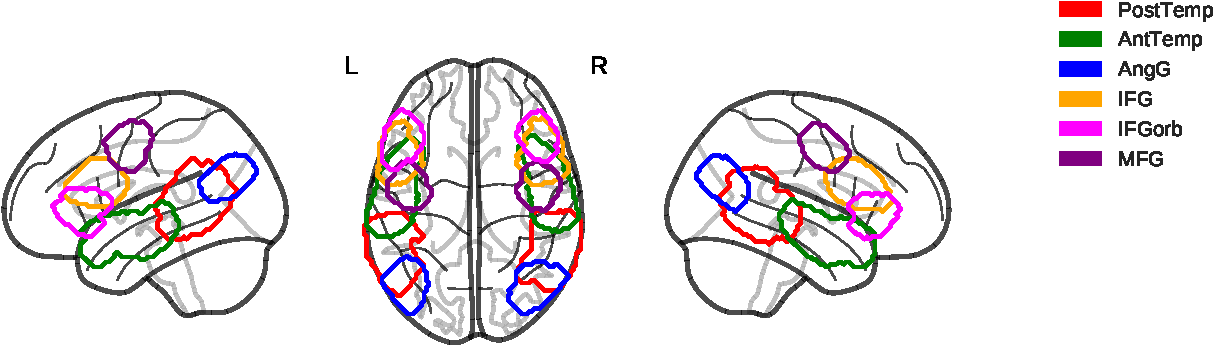
\includegraphics[width=1.0 \linewidth]{figures/part_II/fedorenko_example_img_with_legend.pdf}
\caption{\textbf{Language localizer parcels projected on \emph{Subject 1} anatomy:}
Contours are shown for the projected language localizer parcels reported by Mahowald and Fedorenko.
}
\label{fig:fedorenko_example_img}
\end{figure}


\begin{figure}[hptb]
\centering
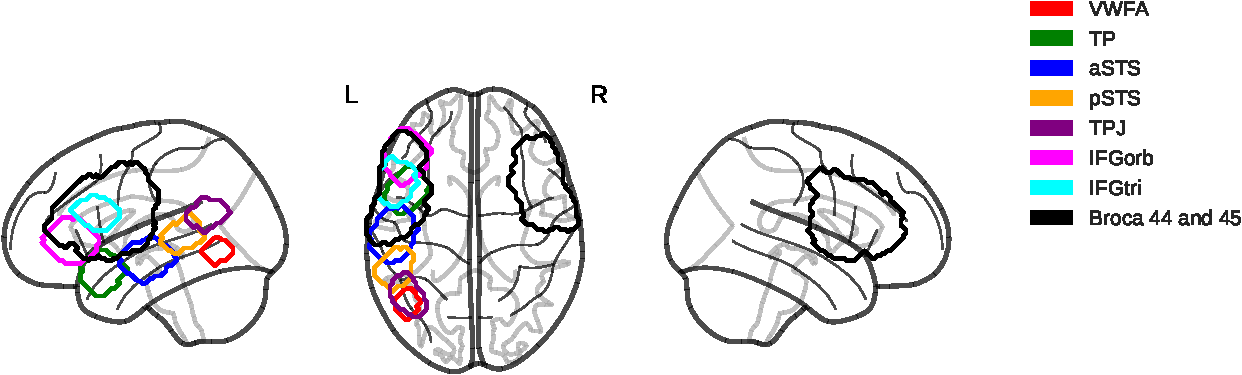
\includegraphics[width=1.0 \linewidth]{figures/part_II/language_example_img_with_legend.pdf}
\caption{\textbf{Language regions of interest projected on \emph{Subject 1} anatomy:}
Contours are shown for the projected left hemispheric language regions of interest. We include the 6 regions reported by Pallier et al. to show phrase constituency effects and the joint Broca 44 and 45 regions taken from the cytoarchitectonic SPM toolbox.
}
\label{fig:langrois_example_img}
\end{figure}


\subsection{Sanity checks}

To verify the integrity of the language localizers acqusitions, we compared the thresholded activations of the constrasts (word sequence over non words sequence), with the parcels of Mahowald and Fedorenko.
These parcels represent likely activation derived from thresholded maps of hundreds of subjects, so not being able to cover them with our language localizer would signal problems with the acqusition and limit our interpretation of syllabic representations in the derived language network.

In the case of the pseudoword matching task runs, we validated the estimated activation maps in two ways.
First we verified the statistical effect of the left vs right motor response contrast and checked that we could decode left and right response activation maps derived from the GLM estimation.
Second we looked for expected retinotopic effects of the centered text in the visual modality, that would imply a separation of the statistical effects of the first syllable position and second syllable position in the right and left hemispheres respectively.


\subsection{Classification and structural tests of representations}

% Never explained motor classification test... was different...
% Should have run motor classification on trial maps....

\paragraph{Classifiers:}
For all classification models we first standardized the activation values in the voxels (features) selected, taking into account activations from the 720 trial maps of each sensory modality.
The standardized features were then passed to a NuSVC linear classifier, for which we performed a grid search for the best value of the "nu" parameter taken from 0.2, 0.5 and 0.8.
We employed the multiclass One Vs Rest (ovr) classification strategy, such that the decision function is based on one classifier per condition.
A Leave One Out Cross Validation (LOOCV) procedure based on sessions was implemented for all trained classifiers.
For estimation of p-values for accuracy and other measurements taken from the classifier, we retrained a model 100 times with shuffled labels.

% Maybe increase permutations to 1000 for final thesis days?

\paragraph{Classification models:}
The final objective was to analyze in Regions of Interest (ROIs) classification of First Position syllables (First model), Second Position (Second model) syllables and Pseudowords (Pseudoword model).
Then chance on the First and Second model was 33.33\% for the three conditions "fi", "gu" and "na", and 11.11\% for the nine pseudoword conditions.
From each classification model we extracted confusion matrices and the model coefficients for further analysis.

\paragraph{Searchlight and voxel selection procedure for ROI analysis:}

% Did not explain ho the region of the searchlight was determined.... by the intersection of langloc 0.001 and any syllable position effect or interaction of 0.001 (where a voxel was considered if any voxel in a sphere radius of 3mm captured such effects)

The ROIs that we considered had thousands of voxels (features), which impacts negatively the performance of classifiers, so we first decided to select promising voxels by running a Searchlight\ref{etzel2013searchlight} classification procedure on a 5 milimiter radius spheres.
We run in each sphere three classifiers: the first position syllable classifier, the second position syllable classifier and the pseudoword classifer.
The classifiers accuracy was assigned to the center voxel of each sphere, resulting in three accuracy maps.
Then voxels from each map were ranked and the top "n" voxels of each map alongise a 3 mm sphere around them were taken as features for the final ROI classifier.
The number "n" of top voxels to consider was cross validated in the parameter grid search of the ROI classifiers, taking values from 1 to 40 in sensory regions and from 1 to 10 in language regions.

% Searchlight was really performed with the avg beta maps of each session
% 

% The center voxels were selected intermitently after masking the images, so one voxel every two, since contigous voxels (features) would be captured by multiple models.
% We expected to identify, in the small spheres, features capable of separating at least some of the classes, so we selected spheres that gave maximum accuracy on the classification of any class and not on overall accuracy.
% The spheres providing the best accuracy for each class were considered together to fit one final model for each ROI.
% We expected the final classifier would be able to distinguish all categories while keeping the number of features as low as possible.
% missing clarification on number of best spheres taken (grid searched?)
% missing clarification on separate feature selection considerations for first and second models vs pseudoword models (only 6 peaks for first and second? 9 for pseudowords? or 15 for all?...)

\paragraph{Implications of the superposition principle:}
The superposition principle predicts that neural representations (voxel activations) should follow Equation \ref{equation:superposition}.
This means that the activation value of a pseudoword at a voxel is the sum of the activation value of a syllable bound to the first position and the activation value of the another syllable bound to the second position.
Then we would expect the representation patterns of pseudowords sharing syllables in the same position to be more similar to each other than completely unrelated pseudowords.
Moreover we would expect pseudowords sharing syllables in different positions to not be more similar to each other than to other unrelated pseudowords, since the neural activity of a syllable is meant to change after being bound to its position.

\begin{equation}
Activation = Syllable \times Position_1 + Syllable \times Position_2 + Noise
\label{equation:superposition}
\end{equation}


\paragraph{Testing superposition with confusion matrices:}
In Figure \ref{fig:super_confusion} we identify each of the cells of a confusion matrix according to the relationship between pseudowords.
Besides the diagonal of the confusion matrix of a classifier representing accuracy, we have three more types of cells: when there is a syllable overlap in some position; when there is a common syllable in a different position; and when there are no common syllables between pseudowords.
The representation similarity structure given by the linear terms in the superposition equation should be reflected in the confusion between conditions in a linear classifier, which means that we can compare the mean confusion of the different cell groups to provide evidence for or against superposed representations.
The principle predicts that the confusion of a position overlap should be higher than that of no overlap while the confusion of a crossed overlap should be no different from that of no overlap.
This means that a positive difference of crossed overlap confusion over no overlap would be evidence against superposition, while a positive difference of position overlap over no overlap would be evidence in favor of superposition.


\begin{figure}[ht]
\scriptsize
\hspace{-4ex}
\begin{tabular}{cl}
{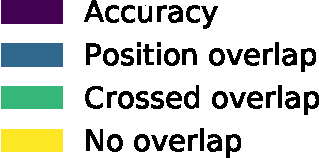
\includegraphics[width=0.3\linewidth]{figures/part_II/super_matrix_legend.pdf}}
\hspace{-1ex}
&{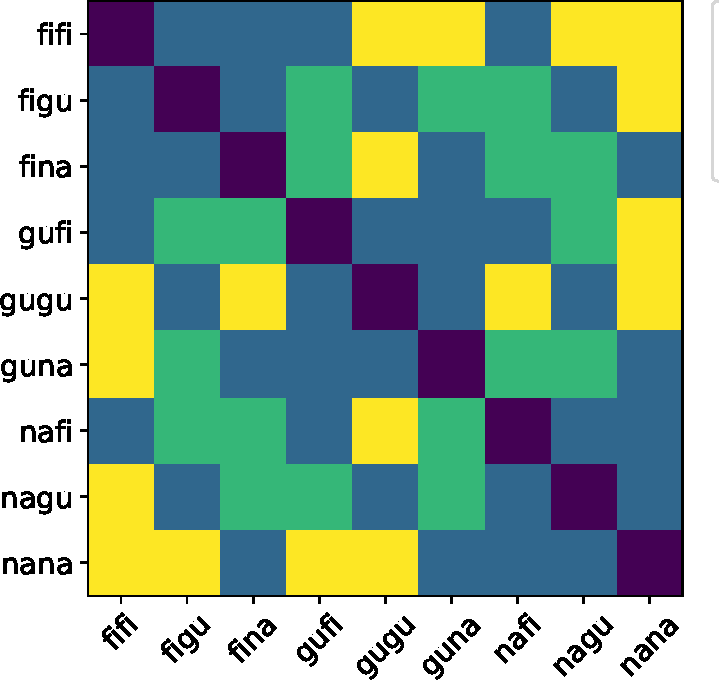
\includegraphics[width=0.6\linewidth]{figures/part_II/super_matrix.pdf}}
\hspace{-1ex}\\
\end{tabular}
\caption{\textbf{Cell types in the confusion matrix of a pseudoword classifier:}
The diagonal represents the classification accuracy of the different pseudowords. The rest of the cells correspond to pseudowords that have an overlapping syllable in one position (Position overlap), a common non overlapping syllable (Crossed overlap) or no common syllables (No overlap).}
\label{fig:super_confusion}
\end{figure}


\paragraph{Partition of syllable position representations:}
We also tested the sparsity of position related representations, which should be fulfilled at least in visual areas due to the hemispheric separation of syllable positions given by retinotopy.
Independently of the possible superposed nature of representations, position encodings could be completely distributed across all voxels or partitioned as in the retinotopic case.
Testing the partition of representations is interesting for the Smolensky's framework that propose the possibility of completely distributed representations.
From the best feature (voxel) coefficients of the linear classifiers of the first position and second position syllables we can get an idea of the level of partition of information in the voxels.
Since a similar subset of voxels is included in both classifiers, we would expect an statistically extreme overlap of the feature rankings, given by the coefficients, in case of distributed representations, while we would expect less overlap than that given by change in case of partitioned representations.
We determined the effects of chance by considering the models trained with shuffled labels, from which we determine the distribution of overlap percentage considering the "n" best voxels of both models for all "n".
An example of the appearance of such a distribution is demonstrated in Figure \ref{fig:segregation_test}


\begin{figure}[ht]
\scriptsize
\hspace{-4ex}
\begin{tabular}{cl}
{
\includegraphics[width=0.3\linewidth]{figures/part_II/example_legend2.pdf}}
\hspace{-1ex}
&{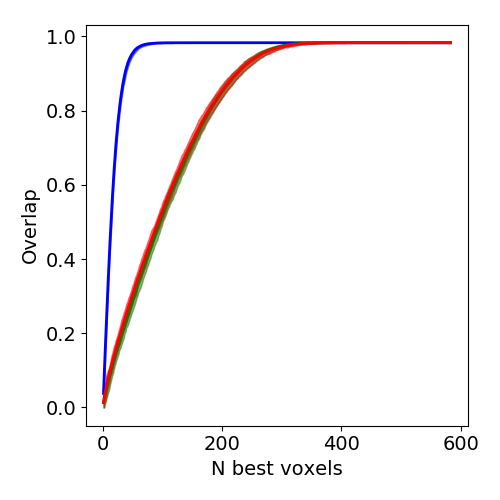
\includegraphics[width=0.6\linewidth]{figures/part_II/theoretical_example2.png}}
\hspace{-1ex}\\
\end{tabular}
\caption{\textbf{Test for partitioned position representations:}
The.}
\label{fig:segregation_test}
\end{figure}
